
\section{Representation}
\label{sec:overview}

Our goal is to learn an animatable virtual characters directly from RGB videos and to support loose clothes like skirts and dresses without pre-scanning a template. To this end, we propose a new representation that has a strong capability of modeling the shape, appearance and dynamic deformations of clothed humans. At its core is a set of \emph{structured local radiance fields}, each of which models the dynamic appearance inside a local space while moving according to the body poses as well as the cloth deformations. 
% Our representation is built upon neural radiance fields~\cite{mildenhall2020nerf}, or NeRF in short, for its excellent performance in learning the appearance of static scenes. To extend NeRF for dynamic character modeling, we break a global NeRF into a set of \emph{structured local radiance fields}, which are uniformly attached to the surface of SMPL model. Each of the local radiance fields is responsible for representing the shape and appearance in the local space around its center. The local radiance fields are driven by the body skeleton, while having their own residual movements. 
% In this way, we model the cloth deformations in a coarse-to-fine manner: the coarsest level is the skeleton motion, the middle level is the residual rigid movements of the local radiance fields, and the finest level is time-varying details inside each local radiance field. An illustration of our representation is presented in Fig.~\ref{fig:reprez}.  [TODO: too long, a little bit confusing, need to polish]
To be more specific, we first pre-define $N$ nodes on the SMPL model via farthest point sampling. Their coordinates on the canonical SMPL surface are denoted with $\{\bm{\bar{n}}_i\}_{i=1}^N$. Since the nodes are sampled from the SMPL model, each of them has an associated skinning weight vector $\bm{\omega}_i\in\mathbb{R}^J$, where $J$ is the number of body joints. 
Given a pose vector $\bm{\theta}^{(t)}$ at time stamp $t$, we can transform node $i$ to the posed space using linear blending skinning (LBS): 
\begin{equation}
\label{eqn:reprez:lbs}
    \bm{\mathrm{T}}_i^{(t)} = \sum \omega_{i,j} \bm{\mathrm{M}}_j(\bm{\theta}^{(t)}), 
\end{equation}
\begin{equation}
\label{eqn:reprez:skinning}
    \bm{n}_i^{(t)} = \bm{\mathrm{T}}_i^{(t)} \bm{\bar{n}}_i, 
\end{equation}
where $\bm{\mathrm{M}}_j(\bm{\theta}^{(t)}) \in SE(3)$ is the rigid transformation of the $j$-th body joints and $\omega_{i,j}$ is the $j$-th entry of $\bm{\omega}_i$. 

In Eqn. (\ref{eqn:reprez:skinning}), the nodes strictly follow the motion of the body surface. In order to handle the non-rigid deformations of clothes, we allow the nodes to shift independently. Mathematically, we assign a time-varying residual translation $\Delta\bm{n}_i^{(t)}$ to node $i$  in the canonical space, and modify Eqn. (\ref{eqn:reprez:skinning}) into:
\begin{equation}
\label{eqn:reprez:skinning_2}
    \bm{n}_i^{(t)} = \bm{\mathrm{T}}_i^{(t)} \left(\bm{\bar{n}}_i + \Delta\bm{n}_i^{(t)}\right).
\end{equation}

Finally, we construct a local radiance field over the influence of each node, with a function $\mathcal{F}_i$ represented by a tiny MLP. This MLP takes as input a coordinate in the local space of node $i$ and outputs a high-dimensional feature vector. To model the fine-grain dynamic details that cannot be represented by node translations, we condition the local radiance field on a dynamic detail embedding $\bm{e}_i^{(t)}$. Formally, given any point $\bm{p}\in\mathbb{R}^3$ in the posed space at frame $t$, we first calculate its coordinate in the local space of node $i$ as:
\begin{equation}
\label{eqn:reprez:local_coord}
    \bm{p}_i = \left(\bm{\mathrm{T}}_i^{(t)}\right)^{-1} \bm{p} - \left(\bm{\bar{n}}_i + \Delta\bm{n}_i^{(t)}\right). 
\end{equation}
After that, we feed it into the local radiance network $\mathcal{F}_i$ and blend the feature vectors produced by all local MLPs:
\begin{equation}
\label{eqn:reprez:feat_fusion}
    \bm{f} = \frac{\sum w_i \mathcal{F}_i(\bm{p}_i; \bm{e}_i^{(t)})}{\sum w_i},  
\end{equation}
where $w_i$ is the blending weight defined as
\begin{equation}
\label{eqn:reprez:blending_weight}
    w_i = \max \{\exp (-\Vert\bm{p} - \bm{n}_i^{(t)}\Vert_2^2 / 2\sigma^2) - \epsilon, 0\}, 
\end{equation}
and $\epsilon$ is a hyperparameter controlling the influence radius of the nodes.
% where $w_i = \max \{\exp (-\Vert\bm{p} - \bm{n}_i^{(t)}\Vert_2^2 / 2\sigma^2) - \epsilon, 0\}$ is the blending weight and $\epsilon$ is a hyperparameter controlling the influence radius of the nodes. 
This blended feature $\bm{f}$ is fed into two additional MLPs, $\mathcal{G}(\cdot)$ and $\mathcal{H}(\cdot)$, to compute the color \& density of $\bm{p}$:
\begin{equation}
\label{eqn:reprez:color_density}
    \mathrm{Color}(\bm{p}) = \mathcal{G}(\bm{f}, \bm{v}), \quad \mathrm{Density}(\bm{p}) = \mathcal{H}(\bm{f}), 
\end{equation}
where $\bm{v}\in\mathbb{R}^3$ is the viewing direction~\cite{mildenhall2020nerf}. 

Overall, the dynamic appearance of a clothed character is parameterized in a coarse-to-fine fashion with three sets of variables: body poses $\{\bm{\theta}^{(t)}\}$, node residual translations $\{\Delta\bm{n}_i^{(t)}\}$ and dynamic detail embeddings $\{\bm{e}_i^{(t)}\}$. With the radiance field determined by these variables and the networks (\textit{i.e.}, $\mathcal{F}_1, \mathcal{F}_2, ..., \mathcal{F}_N$, $\mathcal{G}$ and $\mathcal{H}$), we can shoot rays and render images via volume rendering as in \cite{mildenhall2020nerf}. An illustration of our representation is presented in Fig.~\ref{fig:reprez}. 


\textbf{Discussion. }
Compared to state-of-the-art methods, our representation has two advantages:
\begin{itemize}[leftmargin=*]
\setlength{\itemsep}{0pt}
\setlength{\parsep}{0pt}
\setlength{\parskip}{0pt}
\vspace{-0.2cm}
    \item Our method has expressive representation power in terms of both the motion and the topology. Although the nodes in our representation are sampled from the SMPL model, our method is not restricted by it. Instead, our method allows more degrees of freedom for motion and geometry modeling, enabling avatar creation for different cloth topologies, which is a significant departure from the existing works \cite{peng2021animatable_nerf,neural_actors,Shysheya2019TNR,raj2020anr}. 
    \item Our method does not explicitly define a global canonical field and consequently avoids the need for ``backward skinning" during training. Backward skinning is used to transform the points in the posed space to a global canonical space, and has been the basis of previous methods  \cite{peng2021animatable_nerf,neural_actors,Saito:SCANimate:2021}. Even so, we argue that this operation is ambiguous, especially for the points around contacting body parts. In contrast, our approach computes the radiance of any point in the local space, thus resolving the ambiguity issue. 
    % \item TODOTODOTODO---- capture shadow
\vspace{-0.2cm}
\end{itemize}




\begin{figure}
    \centering
    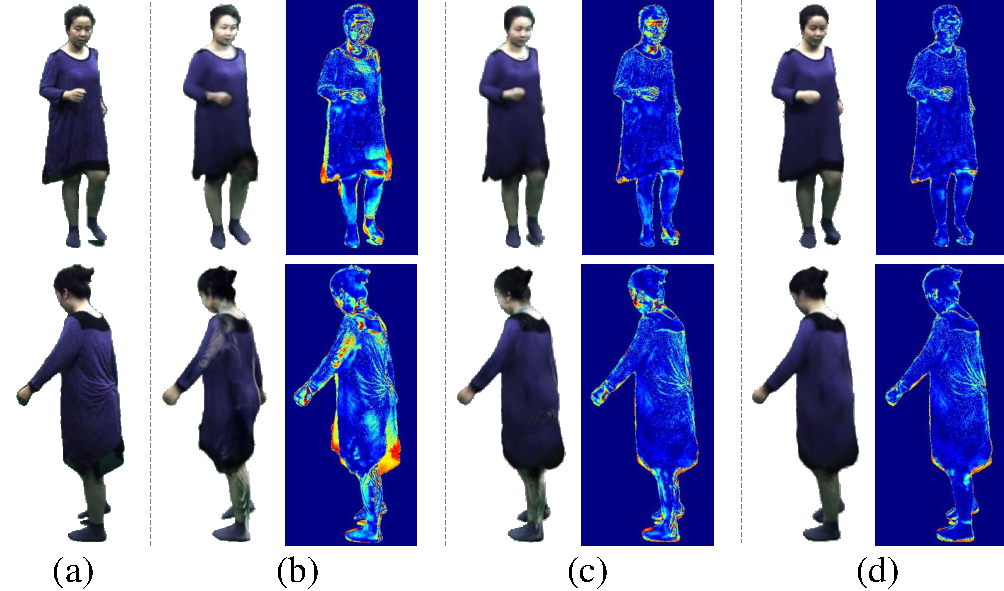
\includegraphics[width=1.0\linewidth]{eval_node_effect}
    \caption{\textbf{Visualization of the effect of node-related variables.} (a) Ground-truth reference. (b) Rendering results without node residual translation and dynamic detail embeddings. (c) Results without dynamic detail embeddings. (d) Results with full set of variables. See Sec.~\ref{sec:experiments:evaluation} for details.}
    \label{fig:eval_node_effect}
\end{figure}




